% Chapter 1
\chapter[TỔNG QUAN VỀ DỮ LIỆU LỚN]
 {\LARGE TỔNG QUAN VỀ DỮ LIỆU LỚN}

% Section 1 Chapter 1
\section{Định nghĩa}
\begin{flushleft}
    Dữ liệu lớn, hay còn được gọi là Big Data, là thuật ngữ chỉ đến tập hợp dữ
    liệu có kích thước lớn hoặc phức tạp đến mức các phương pháp truyền thống
    không đủ để xử lý. Theo định nghĩa của Wikipedia, dữ liệu lớn là một khái
    niệm chỉ đến các tập dữ liệu có quy mô hoặc độ phức tạp đáng kể, đặc biệt
    là khi các phương pháp truyền thống gặp khó khăn trong việc xử lý chúng.\\
    \vspace{0.5cm}
    Tổ chức nghiên cứu Gartner định nghĩa dữ liệu lớn là những nguồn thông tin
    có đặc điểm chung là kích thước lớn, tốc độ xử lý nhanh và định dạng dữ liệu
    đa dạng. Để khai thác hiệu quả dữ liệu lớn, cần áp dụng các phương pháp và
    công nghệ xử lý mới để thực hiện các quyết định, khám phá thông tin mới và
    tối ưu hóa các quy trình.
\end{flushleft}

% Section 2 Chapter 1
\section{Nguồn hình thành của dữ liệu lớn}
Dữ liệu lớn được tạo thành chủ yếu từ 6 nguồn chính, bao gồm:
\begin{itemize}
    \item \textbf{Dữ liệu hành chính}: Phát sinh từ các hoạt động chương trình của tổ chức,
          bao gồm cả chính phủ và phi chính phủ. Ví dụ như hồ sơ y tế điện tử tại các
          cơ sở y tế, hồ sơ bảo hiểm, thông tin ngân hàng.
    \item \textbf{Dữ liệu thương mại}: Xuất phát từ các giao dịch giữa các thực thể kinh
          doanh. Ví dụ như giao dịch thẻ tín dụng, giao dịch trực tuyến, bao gồm cả các
          giao dịch từ thiết bị di động.
    \item \textbf{Dữ liệu từ cảm biến}: Bao gồm thông tin từ các thiết bị cảm biến như
          máy chụp hình vệ tinh, cảm biến đường, cảm biến khí hậu.
    \item \textbf{Dữ liệu từ thiết bị theo dõi}: Bao gồm thông tin thu thập từ các thiết bị
          theo dõi như điện thoại di động, GPS.
    \item \textbf{Dữ liệu từ hành vi trực tuyến}: Bao gồm thông tin từ các hoạt động trực
          tuyến như tìm kiếm sản phẩm, dịch vụ hoặc thông tin khác, cũng như việc đọc
          các trang web.
    \item \textbf{Dữ liệu từ ý kiến và quan điểm}: Bao gồm thông tin về ý kiến, quan điểm
          của cá nhân hoặc tổ chức trên các nền tảng mạng xã hội và các phương tiện
          truyền thông khác.
\end{itemize}
\begin{figure}[ht]
    \centering
    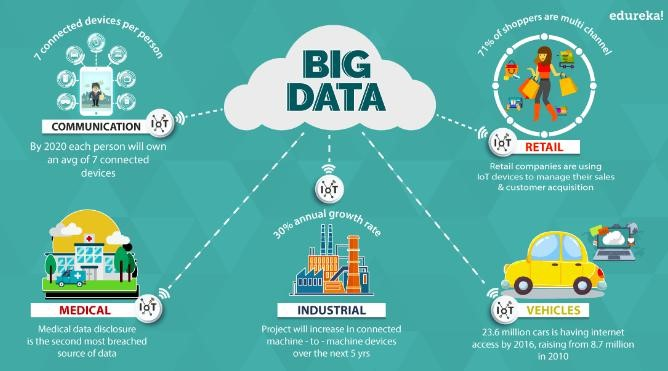
\includegraphics[width=8cm]{images/BigData.jpg}
    \caption{Minh họa nguồn gốc của dữ liệu}
\end{figure}

%Section 3 Chapter 1
\section{Đặc trưng 5V của dữ liệu lớn}
Dữ liệu lớn có 5 đặc điểm cơ bản, được mô hình hóa qua mô hình 5V:
\begin{itemize}
    \item \textbf{Volume (Khối lượng)}: Dữ liệu lớn thường có khối lượng lớn,
          từ hàng terabyte đến petabyte. Để lưu trữ dữ liệu này, chúng ta phải
          sử dụng các công nghệ đám mây mới.
    \item \textbf{Velocity (Tốc độ)}: Dữ liệu lớn được tạo ra và truy cập với
          tốc độ cực kỳ nhanh, đôi khi trong thời gian thực. Điều này đặc biệt quan
          trọng trong các lĩnh vực như Internet, Tài chính, Y tế.
    \item \textbf{Variety (Đa dạng)}: Dữ liệu lớn không chỉ là dữ liệu có cấu trúc
          mà còn bao gồm các loại dữ liệu phi cấu trúc như tài liệu văn bản, hình ảnh,
          video, dữ liệu từ cảm biến vật lý. Việc phân tích và liên kết các loại dữ liệu
          này là thách thức lớn.
    \item \textbf{Veracity (Độ tin cậy/Chính xác)}: DMột trong những vấn đề phức tạp
          nhất của dữ liệu lớn là độ tin cậy và chính xác của dữ liệu. Với sự phát triển
          mạnh mẽ của phương tiện truyền thông xã hội và mạng xã hội, việc đảm bảo tính
          chính xác của dữ liệu trở nên khó khăn hơn.
    \item \textbf{Value (Giá trị)}: Giá trị là yếu tố quan trọng nhất của dữ liệu
          lớn. Trước khi đầu tư vào dữ liệu lớn, chúng ta cần xác định rõ giá trị mà
          thông tin có thể mang lại. Dự báo chính xác và ứng dụng hiệu quả dữ liệu lớn
          có thể mang lại lợi ích lớn, giảm chi phí và tăng hiệu suất trong nhiều lĩnh
          vực.
\end{itemize}

% Section 4 Chapter 1
\section{Tổng quan về Hadoop}
Hadoop là một framework nguồn mở của Apache, viết bằng Java, cho phép
phát triển các ứng dụng phân tán xử lý dữ liệu lớn miễn phí. Nó được
thiết kế để mở rộng từ một máy chủ đơn sang hàng ngàn máy tính khác có
tính toán và lưu trữ cục bộ.
\begin{figure}[ht]
    \centering
    
\includegraphics[width=8cm]{images/Hadoop1.jpg}
    \caption{Biểu tượng của Hadoop}
\end{figure}
\newline
Hadoop có cấu trúc liên kết master-slave, với một node master và nhiều
node slave. Node master gán tác vụ và quản lý tài nguyên, trong khi node slave
lưu trữ dữ liệu thực. Hadoop gồm ba lớp chính:
\begin{itemize}
    \item \textbf{HDFS (Hadoop Distributed File System)}: Hệ thống file phân tán
          của Hadoop, cung cấp khả năng lưu trữ dữ liệu lớn trên nhiều node.
    \item \textbf{MapReduce}: Mô hình lập trình và xử lý dữ liệu song song
          của Hadoop.
    \item \textbf{YARN (Yet Another Resource Negotiator)}: Một hệ thống quản lý
          tài nguyên trong Hadoop.
\end{itemize}
\begin{figure}[ht]
    \centering
    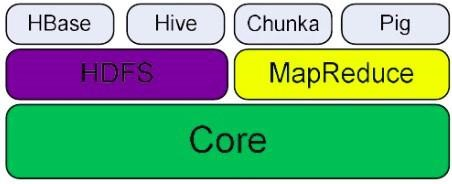
\includegraphics[width=8cm]{images/Hadoop2.jpg}
    \caption{Thành phần của Hadoop}
\end{figure}

% Section 5 Chapter 1
\pagebreak
\section{Tổng quan về MapReduce}
MapReduce là một framework dùng để viết các ứng dụng xử lý song song
một lượng lớn dữ liệu có khả năng chịu lỗi cao xuyên suốt hàng ngàn
cluster (cụm) máy tính.
\vspace{0.5cm}
\newline
MapReduce thực hiện 2 chức năng chính đó là:
\begin{itemize}
    \item \textbf{Map}: Sẽ thực hiện đầu tiên, có chức năng tải,
          phân tích dữ liệu đầu vào và chuyển đổi thành tập
          dữ liệu theo cặp key/value.
    \item \textbf{Reduce}: Sẽ nhận kết quả đầu ra từ tác vụ Map,
          kết hợp dữ liệu lại với nhau thành tập dữ liệu nhỏ hơn, tạo ra
          kết quả cuối cùng.
\end{itemize}
\begin{figure}[ht]
    \centering
    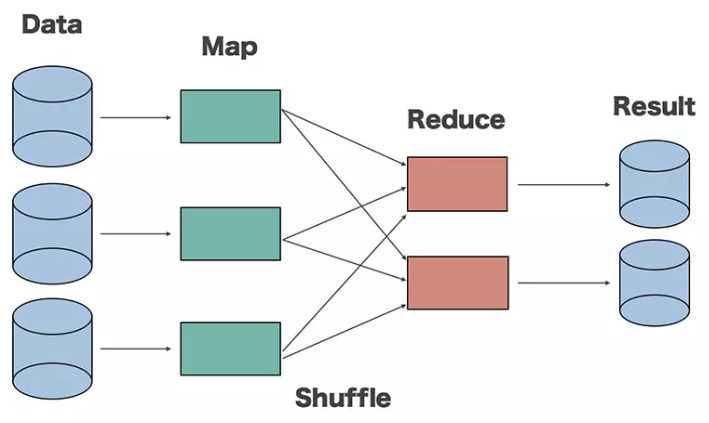
\includegraphics[width=10cm]{images/MapReduce.png}
    \caption{MapReduce}
\end{figure}